\documentclass[a4paper]{ltxdoc}


\usepackage{mlmodern}			% Usa a fonte Latin Modern			
\usepackage[T1]{fontenc}		% seleção de códigos de fonte.
\usepackage[utf8]{inputenc}		% determina a codificação utiizada (conversão automática dos acentos)
\usepackage[brazil]{babel}
\usepackage{hyperref}  			% controla a formação do índice
%\usepackage{parskip}			% espaçamento entre os parágrafos
\usepackage{nomencl} 			% Lista de simbolos
\usepackage{microtype} 			% para melhorias de justificação
\usepackage{booktabs}			% para tabelas
\setlength{\belowcaptionskip}{6pt} % espaçamento depois do título das tabelas
%\setlength{\abovecaptionskip}{6pt}

\hypersetup{
		colorlinks=true,       		% false: boxed links; true: colored links
		linkcolor=blue,        		% color of internal links
		citecolor=blue,        		% color of links to bibliography
		filecolor=magenta,     		% color of file links
		urlcolor=blue}

\IfFileExists{html.sty}
{\usepackage{html}}
{\usepackage{comment}
 \excludecomment{htmlonly}
 \excludecomment{rawhtml}
 \includecomment{latexonly}
 \newcommand{\html}[1]{}
 \newcommand{\latex}[1]{##1}
 \ifx\undefined\hyperref
  \ifx\pdfoutput\undefined \let\pdfunknown\relax
   \let\htmlATnew=\newcommand
  \else
   \ifx\pdfoutput\relax \let\pdfunknown\relax
    \usepackage{hyperref}\let\htmlATnew=\renewcommand
   \else
    \usepackage{hyperref}\let\htmlATnew=\newcommand
   \fi
  \fi
 \else
  \let\htmlATnew=\renewcommand
 \fi
 \ifx\pdfunknown\relax
  \htmlATnew{\htmladdnormallink}[2]{##1}
 \else
  \def\htmladdnormallink##1##2{\href{##2}{##1}}
 \fi
 \long\def\latexhtml##1##2{##1}}

% latex2html nao suporta \ifthenelse...
\usepackage[num,abnt-verbatim-entry=yes]{abntex2cite}
%overcite
%\citebrackets{}

\newcommand{\OKs}{173}
\newcommand{\quaseOKs}{12}
\newcommand{\nadaOK}{3}

\def\Versao$#1 #2${#2}
\def\Data$#1 #2 #3${#2}
%\newcommand{\bibtextitlecommand}[2]{``#2''}

\usepackage{color}
\definecolor{thered}{rgb}{0.65,0.04,0.07}
\definecolor{thegreen}{rgb}{0.06,0.44,0.08}
\definecolor{thegrey}{gray}{0.5}
\definecolor{theshade}{rgb}{1,1,0.97}
\definecolor{theframe}{gray}{0.6}

\IfFileExists{listings.sty}{
  \usepackage{listings}
\lstset{%
	language=[LaTeX]TeX,
	columns=flexible,
	basicstyle=\ttfamily\small,
	backgroundcolor=\color{theshade},
	frame=single,
	tabsize=2,
	rulecolor=\color{theframe},
	title=\lstname,
	escapeinside={\%*}{*)},
	breaklines=true,
	commentstyle=\color{thegrey},
	keywords=[0]{\fichacatalografica,\errata,\folhadeaprovacao,\dedicatoria,\agradecimentos,\epigrafe,\resumo,\siglas,\simbolos,\citacao,\alineas,\subalineas,\incisos},
	keywordstyle=[0]\color{thered},
	keywords=[1]{},
	keywordstyle=[1]\color{thegreen},
	breakatwhitespace=true,
	alsoother={0123456789_},
	inputencoding=utf8,
	extendedchars=true,
	literate={á}{{\'a}}1 {ã}{{\~a}}1 {é}{{\'e}}1 {è}{{\`{e}}}1 {ê}{{\^{e}}}1 {ë}{{\¨{e}}}1 {É}{{\'{E}}}1 {Ê}{{\^{E}}}1 {û}{{\^{u}}}1 {ú}{{\'{u}}}1 {â}{{\^{a}}}1 {à}{{\`{a}}}1 {á}{{\'{a}}}1 {ã}{{\~{a}}}1 {Á}{{\'{A}}}1 {Â}{{\^{A}}}1 {Ã}{{\~{A}}}1 {ç}{{\c{c}}}1 {Ç}{{\c{C}}}1 {õ}{{\~{o}}}1 {ó}{{\'{o}}}1 {ô}{{\^{o}}}1 {Õ}{{\~{O}}}1 {Ó}{{\'{O}}}1 {Ô}{{\^{O}}}1 {î}{{\^{i}}}1 {Î}{{\^{I}}}1 {í}{{\'{i}}}1 {Í}{{\~{Í}}}1,
}
\let\verbatim\relax
 	\lstnewenvironment{verbatim}[1][]{\lstset{##1}}{}
}

\usepackage[T1]{fontenc}		
\usepackage[utf8]{inputenc}		
\usepackage{indentfirst}	

\usepackage{listings}
\usepackage[table,xcdraw]{xcolor}			
\usepackage{graphicx}	
\usepackage{physics}

\usepackage{microtype}
\usepackage{amsfonts}
\usepackage{mathtools}
\usepackage[makeroom]{cancel}

\usepackage{siunitx}
\usepackage{amsthm}
\usepackage{amsmath}
\usepackage{amssymb}

\usepackage{nicematrix} %Matrizes bonitas
\usepackage{tikz}
\usepackage{xkcdcolors} %Cores do xkcd
\usepackage{tikz, tcolorbox, bclogo} %Desenhos e afins
\usepackage{empheq} %Caixas ao redor de equações em um align

\usepackage{float}
\usepackage{caption}
\usepackage{cleveref}
\usepackage{epigraph} 

\usepackage{tabularx}
\usepackage{array}
\usepackage{hyperref}

\numberwithin{equation}{section}
\usepackage{biblatex}

\definecolor{blue}{RGB}{41,5,195}

\frenchspacing




\newtcbox{\mymath}[1][]{%
    nobeforeafter, math upper, tcbox raise base,
    enhanced, colframe=blue!30!black,
    colback=blue!30, boxrule=1pt,
    #1}


\definecolor{shadecolor}{cmyk}{0,0.03,0,0}
\definecolor{light-orange}{cmyk}{0,0.2,0.4,0}
\newsavebox{\mysaveboxM}
\newsavebox{\mysaveboxT}
\newcommand*\Garybox[2][A Nice Box]{%
  \sbox{\mysaveboxM}{#2}%
  \sbox{\mysaveboxT}{\fcolorbox{black}{light-orange}{#1}}%
  \sbox{\mysaveboxM}{%
    \parbox[b][\ht\mysaveboxM+0.5\ht\mysaveboxT+0.5\dp\mysaveboxT][b]{%
      \wd\mysaveboxM}{#2}%
  }%
  \sbox{\mysaveboxM}{%
    \fcolorbox{black}{shadecolor}{%
      \makebox[\linewidth-17.5em]{\usebox{\mysaveboxM}}%
    }%
  }%
  \usebox{\mysaveboxM}%
  \makebox[0pt][r]{%
    \makebox[\wd\mysaveboxM][c]{%
      \raisebox{\ht\mysaveboxM-0.5\ht\mysaveboxT
                +0.5\dp\mysaveboxT-0.5\fboxrule}{\usebox{\mysaveboxT}}%
    }%
  }%
}





\begin{document}


\newcommand{\titulo}{\textbf{Relatório de Lab de Física VI : Gases Ideais}}
\newcommand{\abnTeX}{abn\TeX}

%begin{latexonly}
\title{\titulo}
\author{
Artur Boyago (145599699),
Paulo Azevedo (13839010), \\
João Cruz (13833296)
}
\date{\today}

\maketitle

\begin{abstract}
Resumo dos dados experimentais coletados e analisados no
laboratório de Física VI, lecionado pelo professor Leonardo. O objetivo do experimento
é validar a teoria básica dos gases ideais.
\end{abstract}

\tableofcontents

\section{Caráter teórico do experimento}

\subsection{Parte 1 - Método de Clément-Desormes}

Por meio da relação termodinâmica fundamental é duma equação de estado, se obtém a
equação dos gases ideias:

\begin{align}
    PV=nRT
\end{align}

Sabendo que a constante de gás $\gamma$ é proporcional a potências de $PV$, é experimentalmente possível
encontrar seu valor ao observar uma alteração isotérmica (adiabática):

\begin{align}
    &P_1V_1^\gamma = P_2V_2^\gamma \\
    &\ln \left ( \frac{P_1}{P_2} \right ) +\ln(V_1^\gamma) = \ln(V_2^\gamma)
\end{align}

Com isso podemos ter:

\begin{align}
    \ln \left ( \frac{P_1}{P_2} \right ) &=\gamma \ln(V_2)-\gamma \ln(V_1) \\
    &\rightarrow \ln \left ( \frac{P_1}{P_2} \right ) = \gamma \ln \left ( \frac{V_2}{V_1} \right ) \\
    &\rightarrow \frac {\ln \left ( \frac{P_2}{P_1} \right )}{\ln \left ( \frac{V_1}{V_2} \right ) } = \gamma
\end{align}

Como o processo que ocorre após a o fechamento da válvula é isocórico, temos que $V_2 = V_3$, e como os processos 1 e 3 possuem a mesma temperatura ($T_1 = T_3$), associando à equação dos gases perfeitos, temos:

\begin{align}
    \gamma = \frac {\ln \left ( \frac{P_2}{P_1} \right )}{\ln \left ( \frac{V_1}{V_2} \right ) } 
    = \frac {\ln \left ( \frac{P_2}{P_1} \right )}{\ln \left ( \frac{V_1}{V_3} \right ) } 
    = \frac {\ln \left ( \frac{P_2}{P_1} \right )}{\ln \left ( \frac{ \frac{nRT_1}{P_1} }{\frac{nRT_3}{P_3}} \right ) } 
     = \frac {\ln \left ( \frac{P_2}{P_1} \right )}{\ln \left ( \frac{ \frac{T_1}{P_1} }{\frac{T_1}{P_3}} \right ) } = \rightarrow{} \\
    \rightarrow{} \gamma= \frac {\ln \left ( \frac{P_2}{P_1} \right )}{\ln \left ( \frac{P_3}{P_1} \right ) }
\end{align}


Mas sabemos que as respectivas pressões são:

\begin{align}
    P_1 = P_{atm} \left ( 1 + \frac{\rho g h_1}{P_{atm}}\right  )\\
    P_2 = P_{atm}\\
    P_3 = P_{atm} \left ( 1 + \frac{\rho g h_3}{P_{atm}}\right  )
\end{align}

Portanto temos que:

\begin{align}
    \gamma &= \frac{ \ln \left ( \frac{P_{atm}}{P_{atm} \left ( 1+\frac{\rho g h}{P_{atm}} \right) } \right ) }{ \ln \left ( A \right )} \\
    &= \frac{ \ln(1) - \ln \left ( 1+\frac{\rho g h_1}{P_{atm}} \right ) }{\ln \left ( 1+\frac{\rho g h_3}{P_{atm}}\right )-\ln \left ( 1+\frac{\rho g h_1}{P_{atm}}\right )} \\
    &\approx \frac{h_1}{h_1 - h_3}
\end{align}


\vspace{\baselineskip}

Como o processo inicial é desencadeado após a liberação de parte do gás, que por estar a uma pressão maior que a atmosférica, associada a ao tempo curto dessa liberação, ocasionou uma expansão adiabática do gás restante no recipiente, podemos concluir que, esse restante do gás, por ter efetivamente tendo sofrido as transformações, tando da expansão adiabática quanto o aquecimento isocórico, foi o que efetivamente participou do processo completo.



\subsubsection{Equipamento usado}

\begin{tcolorbox}[colback=white, colframe=red!40!black, title=\textbf{Garrafão de vidro}]
    \begin{tikzpicture} 
        \begin{scope}
            \clip [rounded corners=.5cm] (0,0) rectangle coordinate (centerpoint) (6,6cm); 
            \node [inner sep=0pt] at (centerpoint) {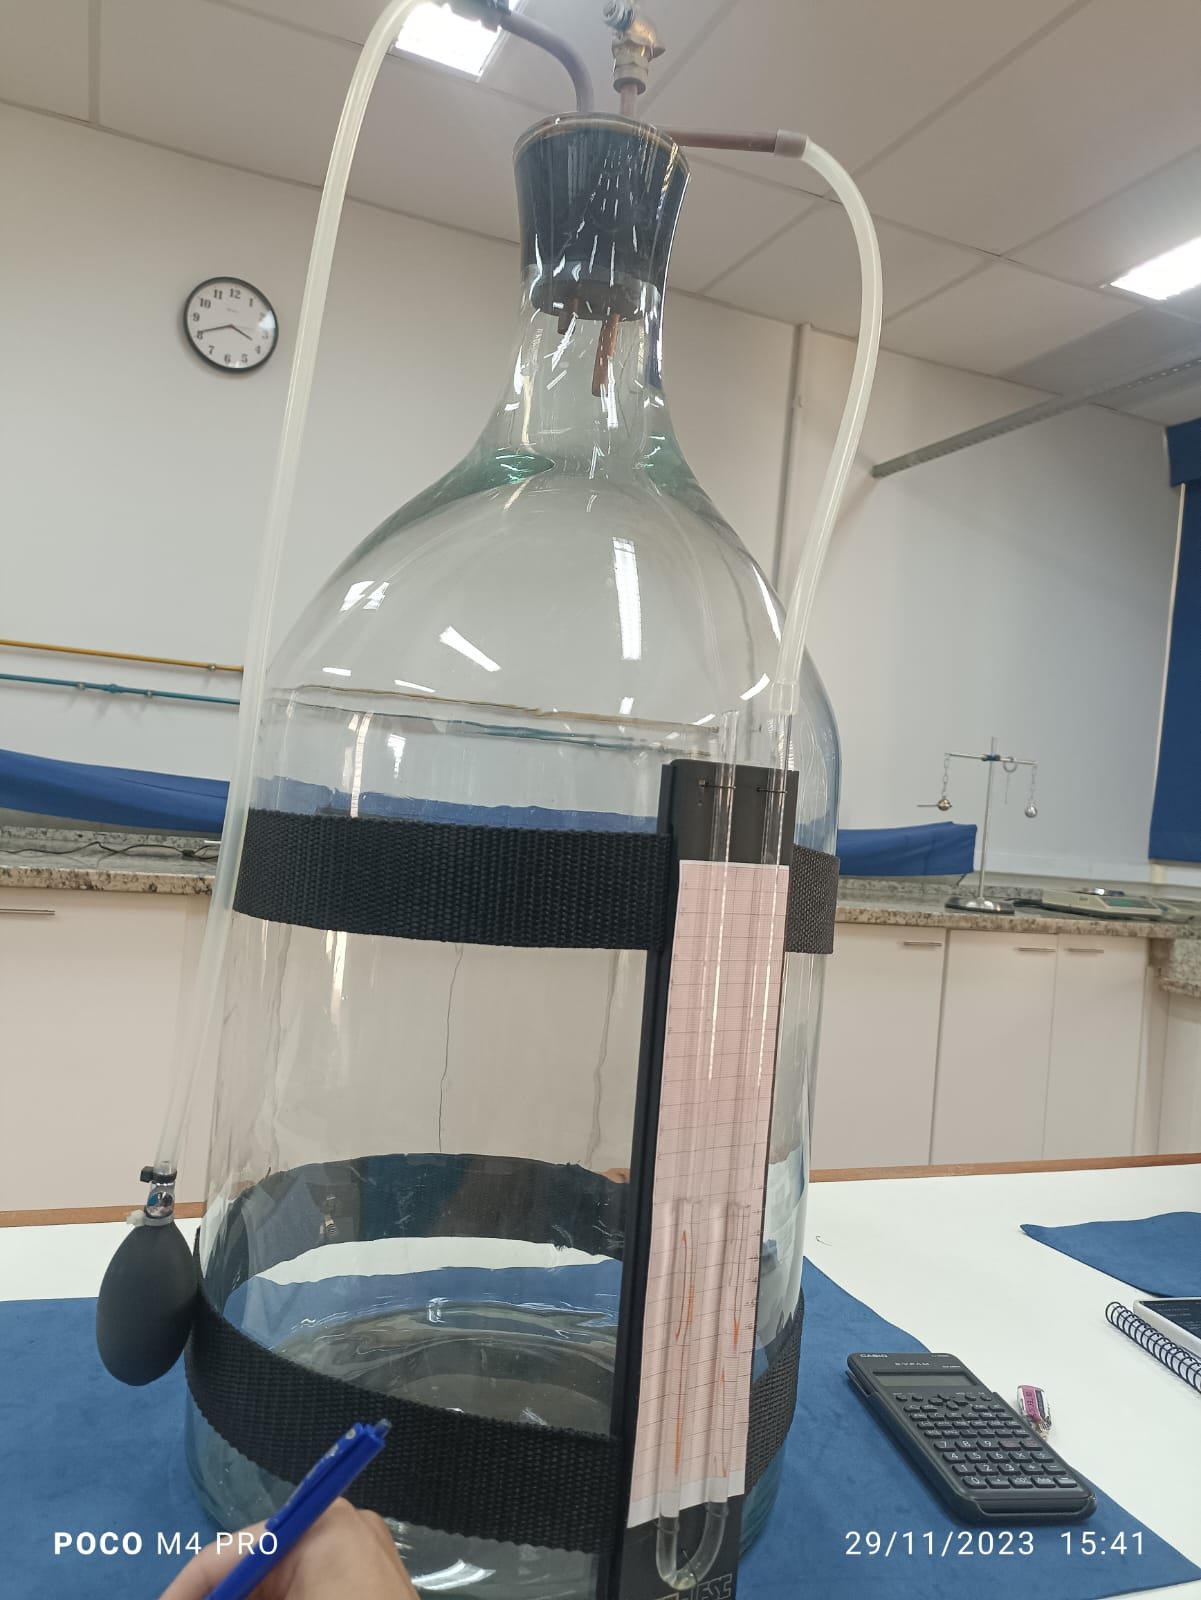
\includegraphics[width=6.0cm]{Garrafao_transformacao_gases.jpg}}; 
        \end{scope}
    \end{tikzpicture}

\end{tcolorbox}


\subsection{Parte 2 - Método de Ruchardt}

Através das características da oscilação do ar provocadas pela esfera, que foram captadas pelo computador, é possível obter as variações de volume e pressão a cada instante, através do cálculo do seu período $T = 2\pi \sqrt{ \frac{Vm}{\gamma PA^2} }$, conseguimos obter o valor de $\gamma$.

\subsection{Parte 3 - Obtenção Zero absoluto}

Para o experimento do zero absoluto é preciso entender como aumentando a temperatura de um gás contido em um recipiente, ele poderá se expandir de diversas maneiras, já que a pressão e o volume podem variar simultaneamente. Evidentemente poderá haver apenas mudança de volume se mantivermos a pressão constante, ou ele exercerá pressões diferentes se o volume for mantido constante. Poderíamos realizar essa expansão colocando o gás em um cilindro fechado por um êmbolo que pode ser deslocado sem atrito, no qual atua uma pressão constante. Experimentalmente pode-se observar que a variação de volume a pressão constante é praticamente proporcional ao volume inicial e a variação de temperatura. Se a temperatura inicial do gás é 0 °C e o seu volume inicial é V0, o volume V(T) a temperatura T °(C) será dado por: 

\vspace{\baselineskip}

\begin{align}
    V(T)=V_0(\beta T + 1)
\end{align}

\vspace{\baselineskip}


Onde é o coeficiente de dilatação do gás a pressão constante. O valor de  é $0,003660 C^{-1} \approx 1273 C^{-1}$ e pode ser considerado como o coeficiente de dilatação dos gases ideais a pressão constante. 
Se agora aumentarmos a temperatura do gás mantido a volume constante, sua pressão deverá variar linearmente com a temperatura. Se a temperatura inicial do gás é $0ºC$ e a sua pressão inicial é P0, a pressão P (T) a temperatura T (C) será dada por:

\begin{align}
    P(T) = P_0(T+1) = P_0T+ P_0
\end{align}

Onde  neste caso é o coeficiente de dilatação a volume constante. Isso pode ser feito pois os coeficientes de dilatação são idênticos para o gás ideal, enquanto que para os gases reais ambos coeficientes são muito próximos a 1/273 (°C)-1 . 

\vspace{\baselineskip}

Substituindo os valores temos: 


\begin{align}
    P(T)=P_0(1 + \frac{T}{273} )
\end{align}

 Neste caso podemos observar que, para $T = - 273 C$, teremos a pressão, P, nula.

 \vspace{\baselineskip}

Para esse experimento do zero absoluto será utilizado um termômetro a gás com volume constante que consiste em um bulbo de vidro com Hélio ligados um barômetro do tipo torricelli. Ou seja, o termômetro é formado por um tubo em “U” contendo mercúrio no seu interior e com um dos braços lacrados para que a pressão no interior do tubo seja zero, no outro braço será colocado um balão de vidro com gás Hélio com uma pressão próxima da pressão atmosférica.

 \vspace{\baselineskip}

Para uma leitura de pressão nesse barômetro, basta observar que a pressão exercida pelo gás He, em um ponto X é exatamente igual à pressão exercida pela coluna de Hg sobre o ponto Y, a qual pode ser obtida diretamente pela altura H (em cm Hg)

 \vspace{\baselineskip}

Durante o experimento será medido a pressão do gás para 4 diferentes temperaturas utilizando os seguintes meio:

%%%
\vspace{\baselineskip}

\begin{itemize}
    \item O bulbo foi mergulhado em água à temperatura ambiente
    \item O bulbo foi mergulhado em gelo em fusão 
    \item O bulbo foi mergulhado em nitrogênio líquido (T= - 196 C)
    \item O bulbo foi mergulhado na água em ebulição
\end{itemize}

\vspace{\baselineskip}
%%%







\section{Parte experimental}


%%%%%%%%%%%%%%%%%%%%%%%%%%%%%%%%%%%%%%%%%%%%%%%%%%%%
\subsection{Parte 1 - Método de Clément-Desormes}

Ao realizar as medidas das alturas das colunas de água nos três estados em questão, obtivemos os seguintes dados:

 \vspace{\baselineskip}

\begin{table}[H]
\begin{tabular}{|c|c|c|c|c|c|}
\hline
\rowcolor[HTML]{FFCCC9} 
Medida 1 & $h_i$ & $h_i'$ & $\Delta h$ & $\gamma$ & $\Delta \gamma$ \\ \hline
Etapa 1  & 9,50  & -9,00  & 18,50      & -        & -               \\ \hline
Etapa 2  & 5,50  & -5,80  & 11,30      & -        & -               \\ \hline
Etapa 3  & 2,00  & -2,10  & 4,10       & -        & -               \\ \hline
Final    & -     & -      & -          & 1,28     & -               \\ \hline
\rowcolor[HTML]{F8A102} 
Medida 2 &       &        &            &          &                 \\ \hline
Etapa 1  & 10,00 & -10,00 & 20,00      & -        & -               \\ \hline
Etapa 2  & 5,50  & -6,00  & 11,50      & -        & -               \\ \hline
Etapa 3  & 3,00  & -3,00  & 6,00       & -        & -               \\ \hline
Final    & -     & -      & -          & 1,43     & -               \\ \hline
\rowcolor[HTML]{F8FF00} 
Medida 3 &       &        &            &          &                 \\ \hline
Etapa 1  & 9,00  & -9,80  & 18,80      & -        & -               \\ \hline
Etapa 2  & 4,80  & -5,20  & 10,00      & -        & -               \\ \hline
Etapa 3  & 2,00  & -2,50  & 4,50       & -        & -               \\ \hline
Final    & -     & -      & -          & 1,31     & -               \\ \hline
\rowcolor[HTML]{6434FC} 
Média    &       &        &            &          &                 \\ \hline
Etapa 1  & 9,50  & -9,60  & 19,10      & -        & -               \\ \hline
Etapa 2  & 5,27  & -5,67  & 10,93      & -        & -               \\ \hline
Etapa 3  & 2,33  & -2,53  & 4,87       & -        & -               \\ \hline
Final    & -     & -      & -          & 1,34     & 0,06            \\ \hline
\end{tabular}
\end{table}

 \vspace{\baselineskip}

Como pudemos observar com os dados obtidos, podemos associar a variação do $\Delta h$ das colunas de água, entre as etapas 1 e 3, ao número de mols de gás que efetivamente participou do processo.

\begin{align}
     \Delta h_1 -\Delta h_3 = P_1 - P_3 = \frac{n_1RT_1} {V} - \frac{n_3RT_3} {V} \xrightarrow[]{T_1 = T_3= T} \\
    \xrightarrow[]{} \Delta h_1 - \Delta h_3 = (n_1 - n_3) \cdot \frac{RT} {V} \xrightarrow[]{} n = n_1 - n_3 = \left ( \Delta h_1 - \Delta h_3 \right ) \cdot \frac{V} {RT} = \\
    = \left (19,10 - 4,87 \right).10^{-2}m \cdot \frac{V .10^{-3}m^3} {8,31 J.mol^{-1}.K^{-1}. 303 K} \xrightarrow[]{} n =  mol
\end{align}







%%%%%%%%%%%%%%%%%%%%%%%%%%%%%%%%%%%%%%%%%%%%%
\subsection{Parte 2 - Método de Ruchardt}

Após realizar o experimento, foi coletado os seguintes dados pelo computador:

\vspace{\baselineskip}

\noindent
\begin{minipage}{\linewidth}
\makebox[\linewidth]{
  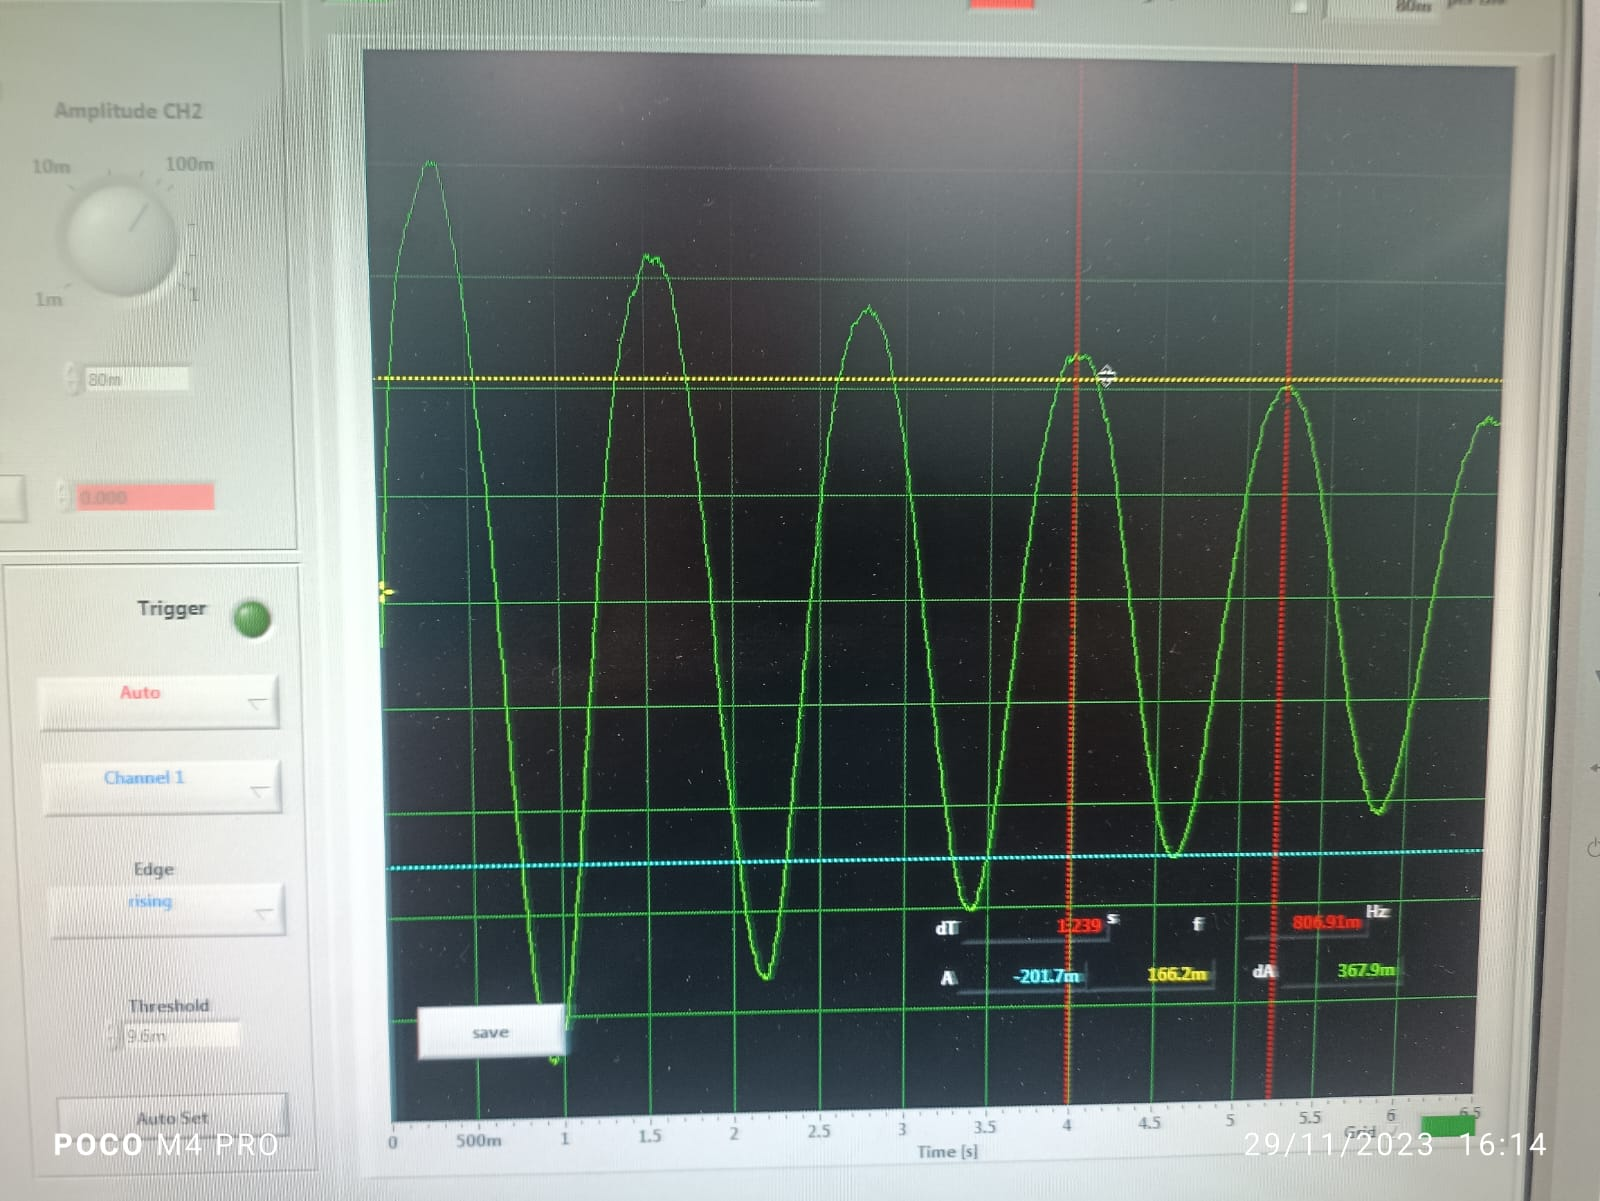
\includegraphics[keepaspectratio=true,scale=0.3]{oscilador.jpg}
  }
\captionof{figure}{
Trajeto de oscilação amortecida do elemento metálico.
}\label{fig:risco1}
\end{minipage}

\vspace{\baselineskip}

\begin{tcolorbox}[colback=white, colframe=blue!40!black, title=\textbf{Tempo de oscilação} ]

O período de oscilação do pequeno objeto será dado por:

\begin{align}
T = 2\pi \sqrt{ \frac{Vm}{\gamma PA^2} }
\label{eq:speed2}
\end{align}

Usando os componentes gráficos, podemos colocar

\end{tcolorbox} 




\subsubsection{Índice $\gamma$}







\begin{tcolorbox}[colback=white, colframe=blue!40!black, title=\textbf{Computando o indice $\gamma$} ]

Isso tudo implica que o coeficiente que define as possíveis condições estacionárias são dadas
quando:

\begin{align}
\gamma \approx \frac{h_1}{h_2-h_3} = \frac{(9,50)}{(9,50) - (2,33)} \approx 1,32 
\end{align}

O que corresponde ao valor monoâtomico observado de Hélio.

\end{tcolorbox} 








%%%%%%%%%%%%%%%%%%%%%%%%%%%%%%%%%%%%%%%%%%%%%%%%%%%%
\subsection{Parte 3 - Obtenção Zero absoluto}

Após a realização dos experimentos, foi obtido os seguintes dados:

\vspace{\baselineskip}

\begin{table}[H]
\begin{tabular}{c|c|c|}
\cline{2-3}
                                                                              & \cellcolor[HTML]{5B9BD5}T (ºC) & \cellcolor[HTML]{5B9BD5}$h_{cm Hg} (cm)$ \\ \hline
\multicolumn{1}{|c|}{\cellcolor[HTML]{FFE699}Água quase fervendo}             & 95,0                             & 88,8                                     \\ \hline
\multicolumn{1}{|c|}{\cellcolor[HTML]{FFE699}Água com   temperatura ambiente} & 24,4                             & 81,3                                     \\ \hline
\multicolumn{1}{|c|}{\cellcolor[HTML]{FFE699}Água com gelo   em fusão}        & 7,3                              & 79,3                                     \\ \hline
\multicolumn{1}{|c|}{\cellcolor[HTML]{FFE699}Nitrogênio   líquido}            & -196,0                           & 56,0                                     \\ \hline
\end{tabular}
\end{table}

\vspace{\baselineskip}

A partir dessa tabela, podemos construir o seguinte gráfico:

%%%
\vspace{\baselineskip}

\noindent
\begin{minipage}{\linewidth}
\makebox[\linewidth]{
  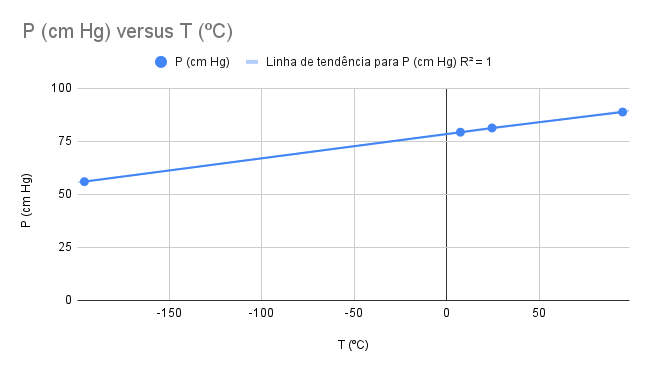
\includegraphics[keepaspectratio=true,scale=0.3]{P-(cm-Hg)-versus-T(C).png}
  }
\captionof{figure}{
Linha de relação entre temperaturas (eixo horizontal) e a altura da coluna de mercúrio (eixo vertical). O valor previsto do zero absoluto é a interseção dessa linha com o eixo horizontal.
}\label{fig:risco1}
\end{minipage}

\vspace{\baselineskip}
%%%






 \vspace{\baselineskip}
 
\begin{thebibliography}{9}
\bibitem{Azuela} Jose F. Schneider, \textit{Laboratório de Física II : Livro de práticas}, USP (São Carlos, IFSC, 2017).
\bibitem{Azuela} Schroeder D.V, \textit{Introduction to Thermal Physics}
\end{thebibliography}


\end{document}